\documentclass{beamer}

\usepackage[utf8]{inputenc}
\usepackage[ngerman]{babel}
\usepackage{minted}
\usepackage{hyperref}
\usepackage{color}

\usemintedstyle{emacs}

\usetheme[progressbar=head,block=fill]{metropolis}
\title{Porting Software To Genode}
\date{July 11, 2017}
\author{Alexander Weidinger}
\institute{Technische Universität München}
\begin{document}
  \maketitle

  \begin{frame}{Overview}
    \begin{itemize}
      \item Native port of an application or library
      \item (Using Genode's Noux runtime)
      \item (Porting device drivers)
    \end{itemize}
  \end{frame}

  \begin{frame}{Steps}
    \begin{enumerate}
      \item Look up dependencies
      \item Writing a \textit{*.port} file
      \item Writing a \textit{*.mk} file
      \item Compilation
      \item Testing
    \end{enumerate}
  \end{frame}

  \begin{frame}{Filesystem Structure Genode-World}
    \begin{itemize}
      \item src \textcolor{gray}{\textit{(source code or patch files incl. *.mk files)}}
      \begin{itemize}
        \item app
        \item lib
        \item test
        \item ...
      \end{itemize}
      \item lib \textcolor{gray}{\textit{(*.mk files for libs incl. import-mk files)}}
      \begin{itemize}
        \item import
        \item mk
      \end{itemize}
      \item ports \textcolor{gray}{\textit{(*.hash and *.port files)}}
      \item run \textcolor{gray}{\textit{(*.run files)}}
    \end{itemize}
  \end{frame}

  \section{libmosquitto}

  \begin{frame}[fragile]{\textit{*.port} And \textit{*.hash} Files}
    \begin{block}{ports/libmosquitto.port}
      \begin{minted}[fontsize=\tiny]{bash}
VERSION   := 1.4.12
DOWNLOADS := mosquitto.archive
LICENSE   := EPL

URL(mosquitto) := https://mosquitto.org/files/source/mosquitto-$(VERSION).tar.gz
SHA(mosquitto) := 1451547e56bf4d33ea156cbc21f1d12acb58318b
DIR(mosquitto) := src/lib/libmosquitto

PATCHES := src/lib/libmosquitto/net_mosq.patch
      \end{minted}
    \end{block}

    \begin{block}{ports/libmosquitto.hash}
      \begin{minted}[fontsize=\tiny]{bash}
c12001a88ffc6f51cc5f8e23e50078eb4e2ce5cc
      \end{minted}
    \end{block}
  \end{frame}

  \begin{frame}[fragile]{target.mk file}
    \begin{block}{lib/mk/libmosquitto.mk}
      \begin{minted}[fontsize=\tiny]{makefile}
LIBMOSQUITTO_DIR := $(call select_from_ports,libmosquitto)/src/lib/libmosquitto

SRC_LIBMOSQUITTO := logging_mosq.c memory_mosq.c messages_mosq.c mosquitto.c \
        net_mosq.c read_handle.c read_handle_client.c read_handle_shared.c \
        send_client_mosq.c send_mosq.c socks_mosq.c srv_mosq.c thread_mosq.c \
        time_mosq.c tls_mosq.c util_mosq.c will_mosq.c

INC_DIR += $(LIBMOSQUITTO_DIR) $(LIBMOSQUITTO_DIR)/lib $(LIBMOSQUITTO_DIR)/lib/cpp/

SRC_CC = $(addprefix $(LIBMOSQUITTO_DIR)/lib/, $(SRC_LIBMOSQUITTO)) \
         $(LIBMOSQUITTO_DIR)/lib/cpp/mosquittopp.cpp

LIBS += libc libc_lwip lwip pthread stdcxx libssl

CC_DEF += -DWITH_TLS -DWITH_TLS_PSK -DWITH_EC -DWITH_SOCKS -DWITH_THREADING

SHARED_LIB = yes

CC_OPT += -O2
      \end{minted}
    \end{block}
  \end{frame}

  \begin{frame}[fragile]{import.mk file}
    \begin{block}{lib/import/import-libmosquitto.mk}
      \begin{minted}[fontsize=\tiny]{makefile}
LIBMOSQUITTO_PORT_DIR := $(call select_from_ports,libmosquitto)
INC_DIR += $(LIBMOSQUITTO_PORT_DIR)/src/lib/libmosquitto/lib/ \
           $(LIBMOSQUITTO_PORT_DIR)/src/lib/libmosquitto/lib/cpp
      \end{minted}
    \end{block}
  \end{frame}

  \begin{frame}[fragile]{Testing}
    \begin{itemize}
      \item Write an application, which makes use of the library
      \uncover<2->{\item Compile and run it}
      \uncover<3->{\item Hope for the best}
      \uncover<5->{\item Write patches, port additional libraries, ...}
    \end{itemize}
    \uncover<4->{
      \begin{figure}
        
\includegraphics[scale=0.2]{img/this_is_fine.png}\tiny\footnote<4->{\tiny\url{http://knowyourmeme.com/memes/this-is-fine}}
      \end{figure}
    }
  \end{frame}

  \begin{frame}[fragile]{Problems With Libmosquitto}
    \begin{exampleblock}{Missing implementations}
      \begin{minted}[fontsize=\tiny]{text}
[init -> mpct] int socketpair(int, int, int, int*): socketpair not implemented
      \end{minted}
    \end{exampleblock}
    \begin{exampleblock}{Double initializations}
      \begin{minted}[fontsize=\tiny]{c}
Plugin::Plugin() {
  Genode::log("using the lwIP libc plugin");
  lwip_tcpip_init();
}
      \end{minted}
    \end{exampleblock}
  \end{frame}

  \begin{frame}[fragile]{Patches For Libmosquitto}
    \begin{block}{src/lib/libmosquitto/net\_mosq.patch}
      \begin{minted}[fontsize=\tiny]{diff}
+++ src/lib/libmosquitto/lib/net_mosq.c
@@ -1172,7 +1172,6 @@ int _mosquitto_socket_nonblock(mosq_sock_t sock)
 #ifndef WITH_BROKER
 int _mosquitto_socketpair(mosq_sock_t *pairR, mosq_sock_t *pairW)
 {
-#ifdef WIN32
 	int family[2] = {AF_INET, AF_INET6};
 	int i;
 	struct sockaddr_storage ss;
@@ -1278,25 +1277,5 @@ int _mosquitto_socketpair(mosq_sock_t *pairR, mosq_sock_t *pairW)
 		return MOSQ_ERR_SUCCESS;
 	}
 	return MOSQ_ERR_UNKNOWN;
-#else
-	int sv[2];
-
-	if(socketpair(AF_UNIX, SOCK_STREAM, 0, sv) == -1){
-		return MOSQ_ERR_ERRNO;
-	}
@@[...]
-	*pairR = sv[0];
-	*pairW = sv[1];
-	return MOSQ_ERR_SUCCESS;
-#endif
 }
 #endif
      \end{minted}
    \end{block}
  \end{frame}

  \begin{frame}{References}
    \begin{enumerate}
      \item \href{https://genode.org/documentation/developer-resources/porting}{Genode Porting Guide: Overview}
      \item \href{https://github.com/prurigro/intelligent-snake}{A simple snake clone in C and SDL 1.2}
    \end{enumerate}

    \begin{figure}
      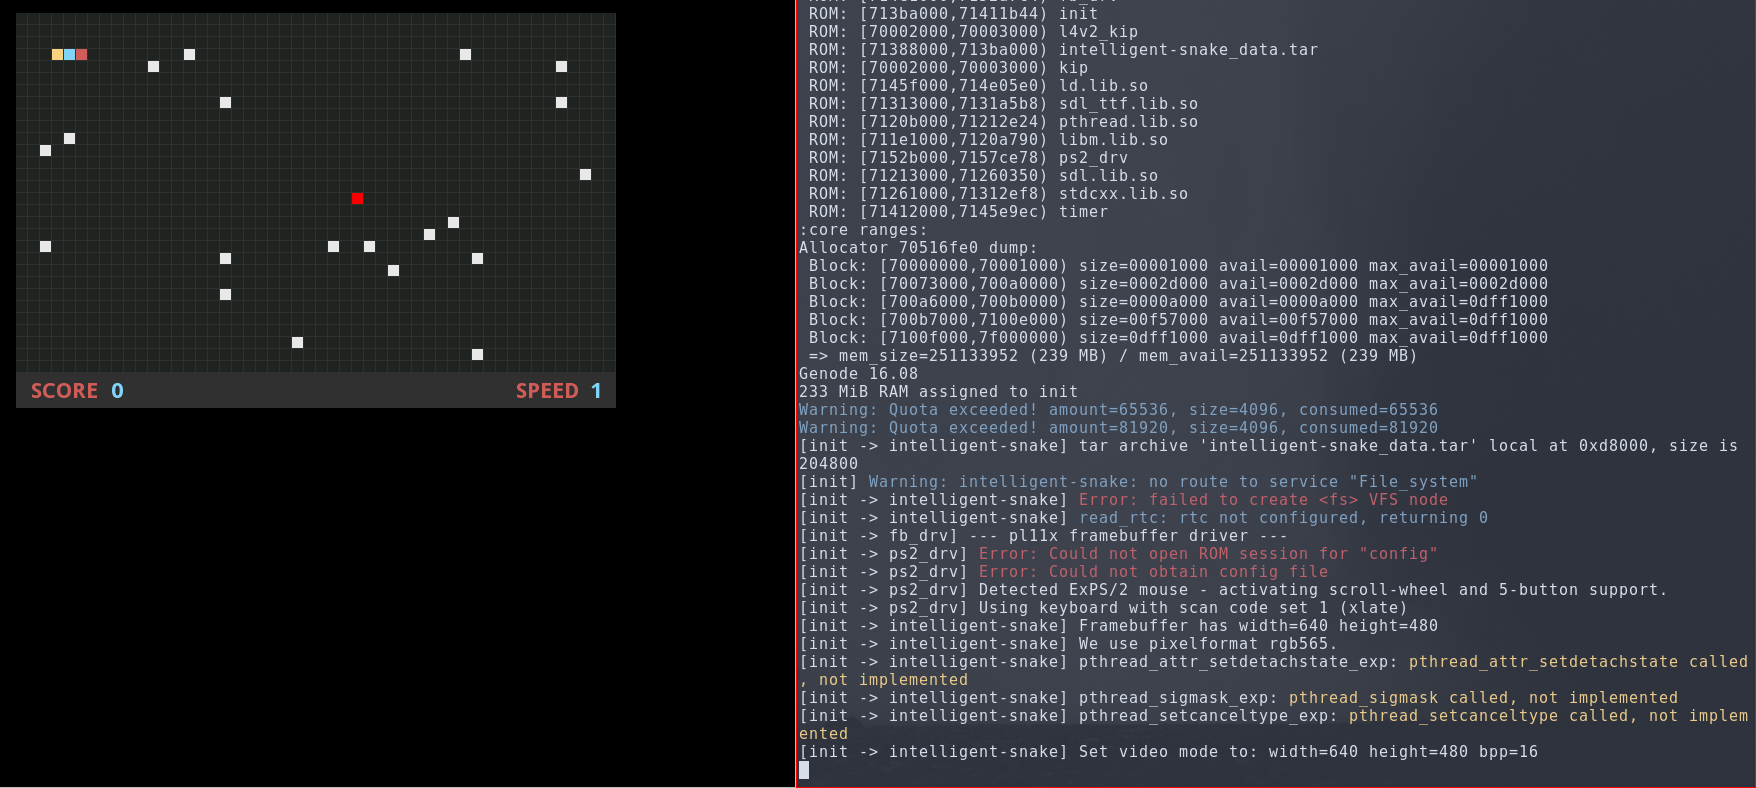
\includegraphics[scale=0.15]{img/isnake.png}
    \end{figure}
  \end{frame}
\end{document}
